\documentclass[varwidth=\maxdimen,border=0pt]{standalone}
\renewcommand{\sfdefault}{phv}

 \renewcommand{\familydefault}{\sfdefault}
%\fontfamily{helvetica}
  %\selectfont


\usepackage{subcaption}
\usepackage[labelformat=parens,labelsep=quad,skip=3pt]{caption}
\usepackage{graphicx}
\usepackage[export]{adjustbox}
\usepackage{xcolor}

\definecolor{gray90}{HTML}{F8F8F8	}

\newcommand{\subfigimg}[3][,]{%
  \setbox1=\hbox{\includegraphics[#1]{#3}}% Store image in box
  \leavevmode\rlap{\usebox1}% Print image
  \rlap{\hspace*{0pt}\raisebox{\dimexpr\ht1-\baselineskip}{#2}}% Print label
  \phantom{\usebox1}% Insert appropriate spcing
}

\newcommand{\subfigimga}[4][,]{%
  \setbox1=\hbox{\includegraphics[#1]{#4}}% Store image in box
  \leavevmode\rlap{\usebox1}% Print image
  \rlap{\hspace*{0pt}\raisebox{.975\dimexpr\ht1}{#2}}% Print label
  \rlap{\hspace*{0pt}\raisebox{.55\dimexpr\ht1}{#3}}% Print label
  \phantom{\usebox1}% Insert appropriate spcing
}

\newcommand{\subfigimgb}[3][,]{%
  \setbox1=\hbox{\includegraphics[#1]{#3}}% Store image in box
  \leavevmode\rlap{\usebox1}% Print image
  \rlap{\hspace*{0pt}\raisebox{.975\dimexpr\ht1}{#2}}% Print label
  \phantom{\usebox1}% Insert appropriate spcing
}

\newcommand{\subfigimgc}[3][,]{%
  \setbox1=\hbox{\includegraphics[#1]{#3}}% Store image in box
  \leavevmode\rlap{\usebox1}% Print image
  \rlap{\hspace*{0pt}\raisebox{.975\dimexpr\ht1-1.5\baselineskip}{#2}}% Print label
  \phantom{\usebox1}% Insert appropriate spcing
}

\begin{document}    

\begin{figure}

    \begin{subfigure}[htb]{9cm}
        \subfigimg[width=8.7cm,left]{A.}{../../figures/analysis/map.pdf} 
    \end{subfigure}%
        \begin{subfigure}[htb]{6cm}
             \subfigimga[width=6cm]{B.}{C.}{../../figures/analysis/precip.pdf} % 
               \subfigimgc[width=6cm]{D.}{../../figures/analysis/zero-fitness.pdf}  
      % \colorbox{gray90}{\subfigimgb[width=5.5cm]{E.}{../../figures/analysis/simulation-1.pdf}%<---
     %  }
     %  \colorbox{gray90}{\subfigimgb[width=5.5cm]{F.}{../../figures/analysis/simulation-2.pdf}%<---
      % } 
   	\end{subfigure}
      \end{figure}
      
      
%\begin{figure}
%
%    \begin{subfigure}[t]{6cm}
%        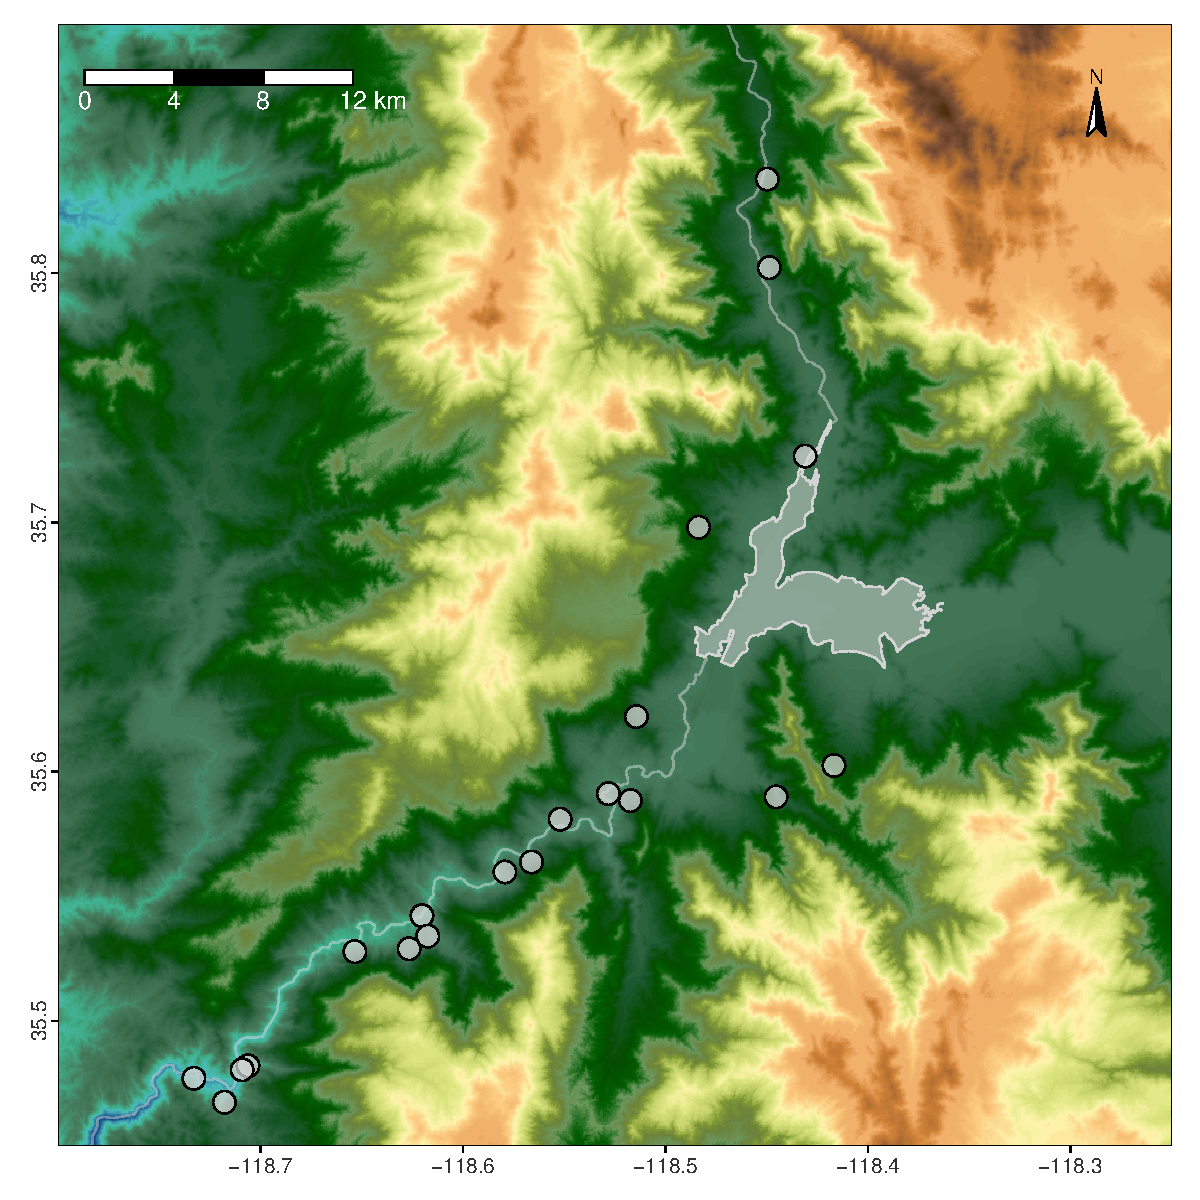
\includegraphics[width=5.7cm,right]{../../figures/analysis/map.pdf} 
%        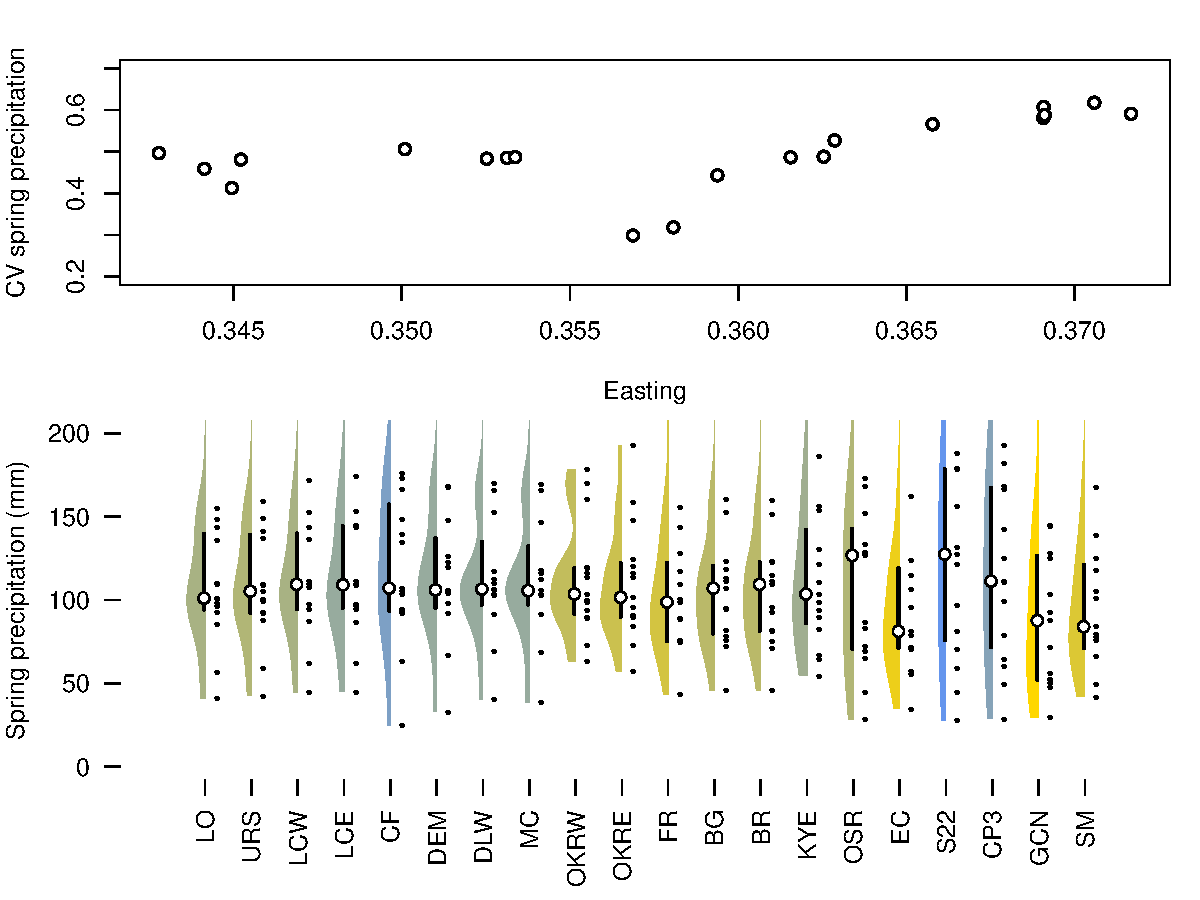
\includegraphics[width=6cm]{../../figures/analysis/precip.pdf} 
%    \end{subfigure}%
%        \begin{subfigure}[t]{6cm}%
%       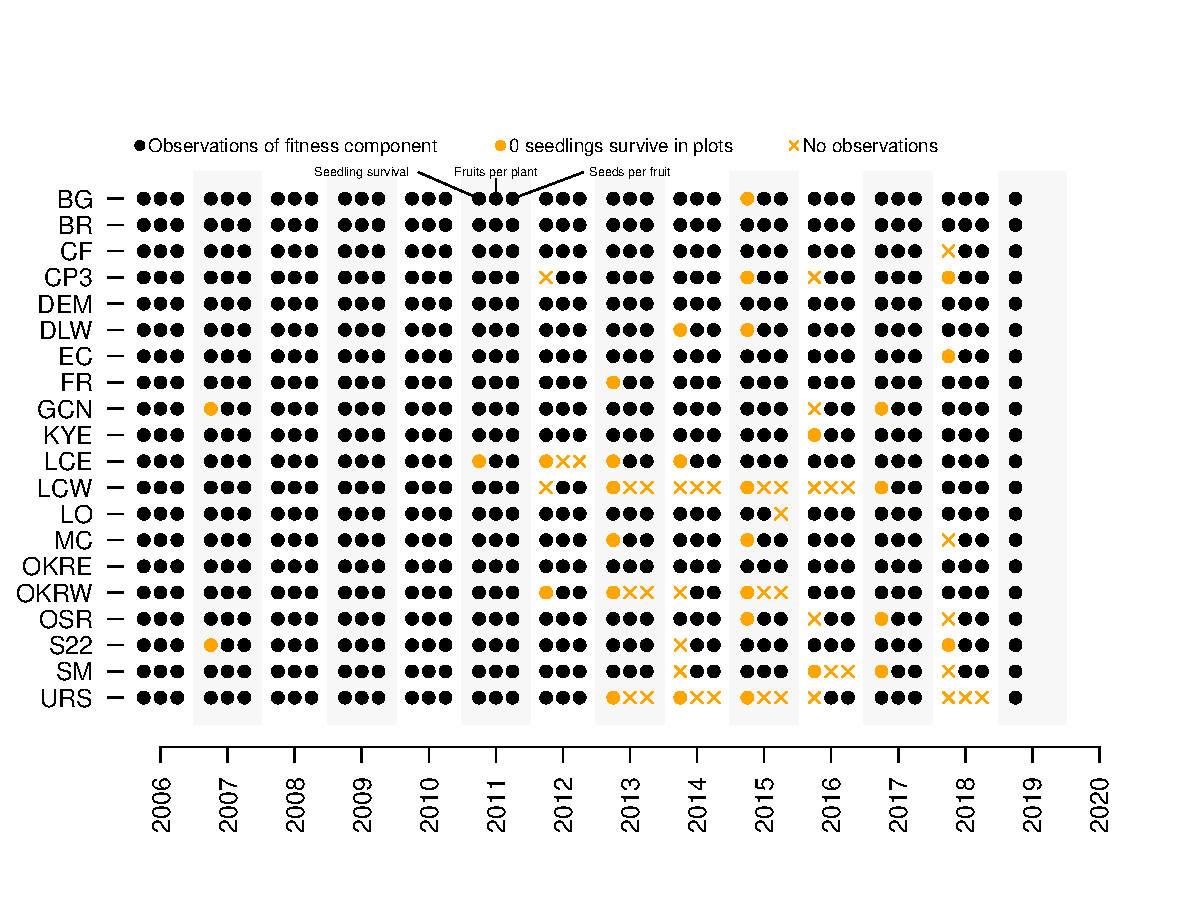
\includegraphics[width=6cm]{../../figures/analysis/zero-fitness.pdf}  
%       \colorbox{gray90}{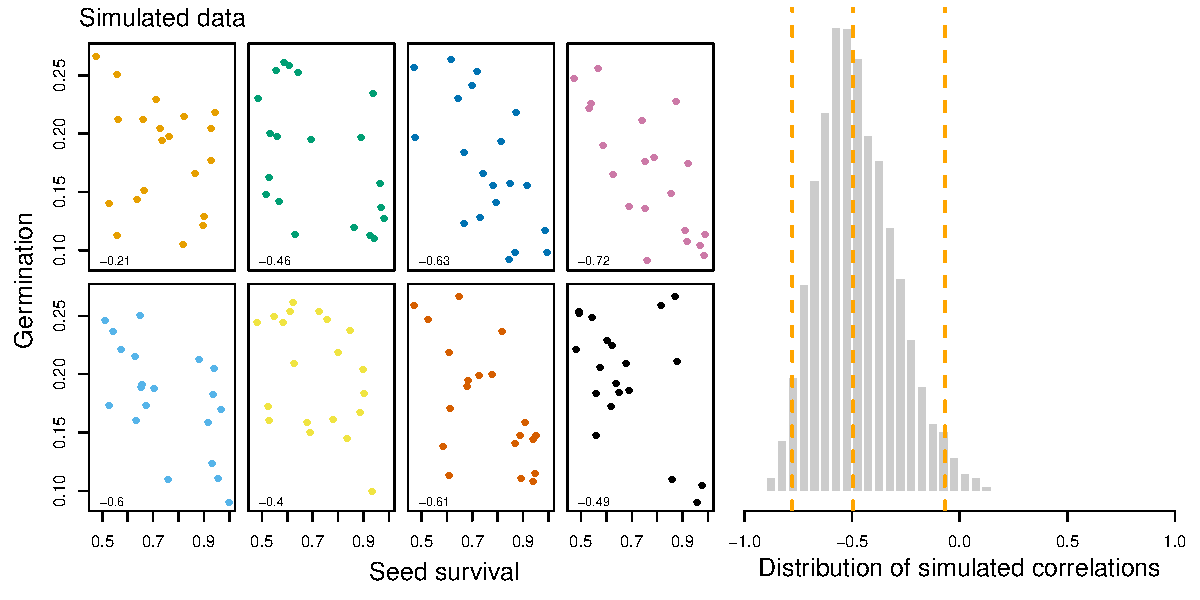
\includegraphics[width=5.5cm]{../../figures/analysis/simulation-1.pdf}%<---
%       }
%       \colorbox{gray90}{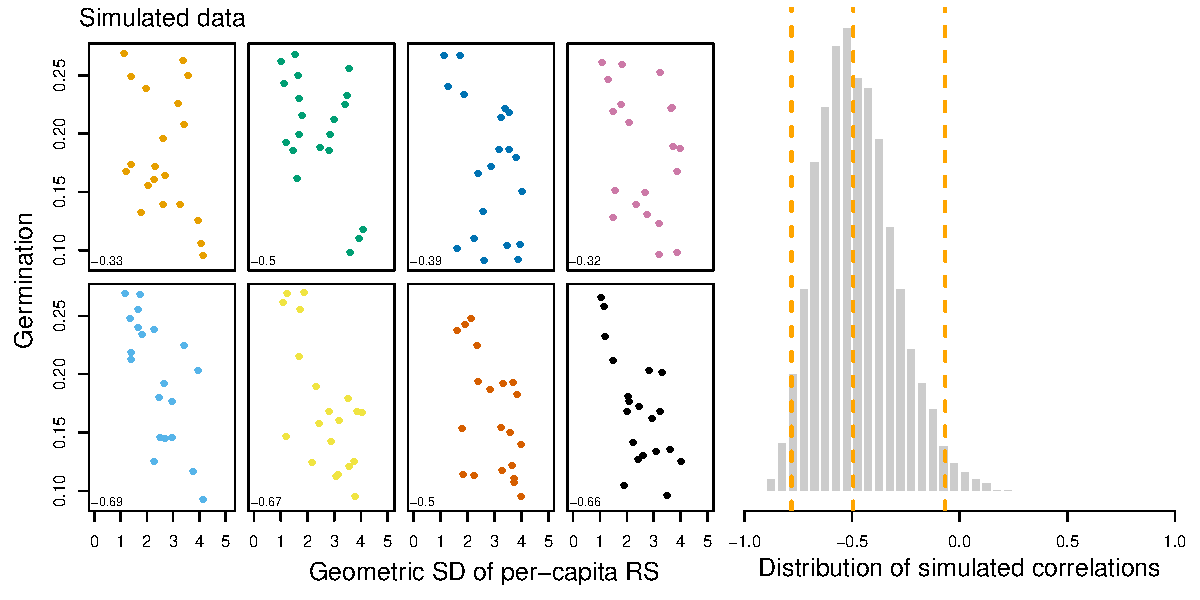
\includegraphics[width=5.5cm]{../../figures/analysis/simulation-2.pdf}%<---
%       } 
%   	\end{subfigure}
%      \end{figure}
      
      
  
  \end{document}